The paper~\cite{kolosov2025efficient} describes a remarkable result that follows
from the odd power identity~\eqref{theorem:odd-power-identity}.
As revealed, by introducing an additional parameter for upper summation bound in $k$
to~\eqref{theorem:odd-power-identity}, the resulting family of polynomials
approximate the odd power in some neighborhood of a fixed point.
\begin{align*}
    P(m,X,N) = \sum_{r=0}^{m} \sum_{k=1}^{N} \coeffA{m}{r} k^r (X-k)^r
\end{align*}
For example,
\begin{align*}
    P(2,X,0) &= 0 \\
    P(2,X,1) &= 30X^2 - 60X + 31 \\
    P(2,X,2) &= 150X^2 - 540X + 512 \\
    P(2,X,3) &= 420X^2 - 2160X + 2943 \\
    P(2,X,4) &= 900X^2 - 6000X + 10624
\end{align*}
The following plot demonstrates the approximation of fifth power $X^5$ by
$P(2,X,4) = 900X^2 - 6000X + 10624$
\begin{figure}[H]
    \centering
    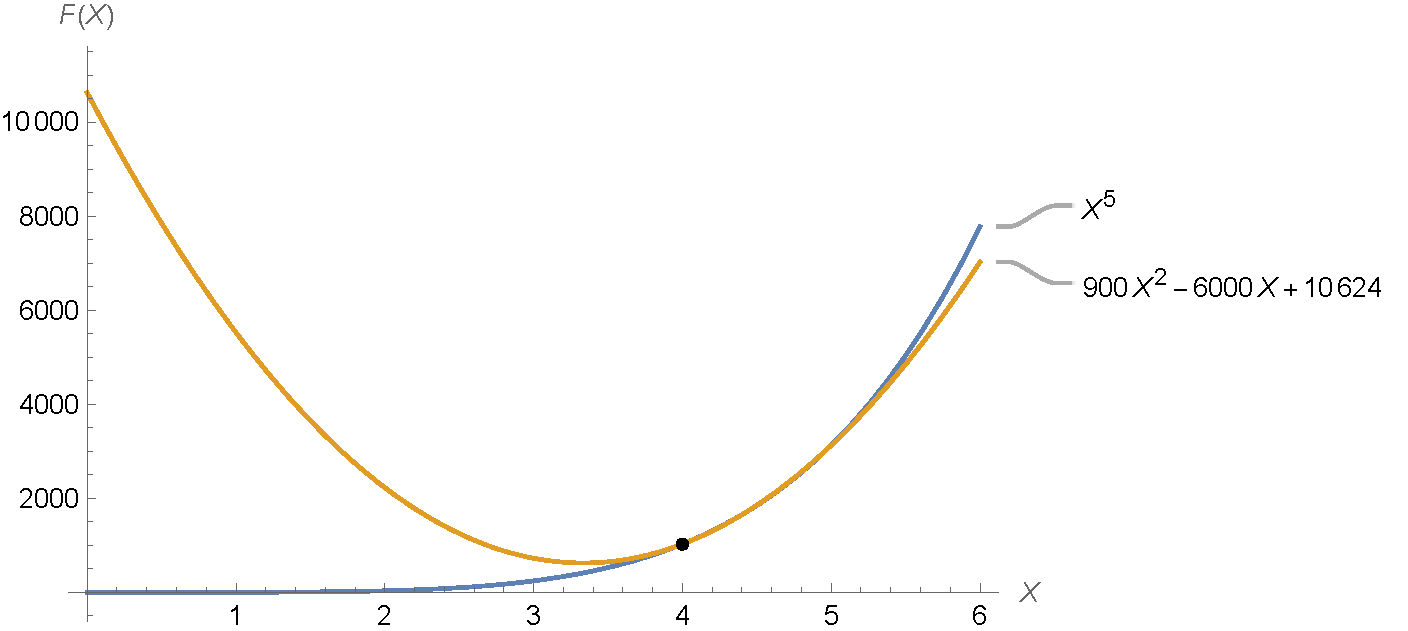
\includegraphics[width=1\textwidth]{sections/images/03_plots_polynomial_p2_n4_with_fifth}
    ~\caption{Approximation of fifth power $X^5$ by $P(2, X, 4)$.
    Convergence interval is $4.0 \leq X \leq 5.1$ with a percentage error $E < 1\%$.
    }\label{fig:03_plots_polynomial_p2_n4_with_fifth}
\end{figure}
Another remarkable observation is
One more interesting observation arises by increasing the value of $N$ in $P(m, X, N)$ while keeping $m$ fixed.
As $N$ increases, the length of the convergence interval with the odd-power $X^{2m+1}$ also increases.
For instance,
\begin{itemize}
    \item For $P(2, X, 4)$ and $X^5$, the convergence interval with a percentage error less than $1\%$ is $4.0 \leq X \leq 5.1$, with a length $L=1.1$
    \item For $P(2, X, 20)$ and $X^5$, the convergence interval with a percentage error less than $1\%$ is $18.7 \leq X \leq 22.9$, with a length $L=4.2$
    \item For $P(2, X, 120)$ and $X^5$, the convergence interval with a percentage error less than $1\%$ is $110.0 \leq X \leq 134.7$, with a length $L=24.7$
\end{itemize}
